\part{Analyse des données textuelles}

    \chapter{Caractéristiques générales du jeu de données}

        Dans toute cette analyse, on se basera sur les données manuellement étiquetées (ou ground truth), échantillon de 500 fiches techniques avec les listes d'ingrédients associées.

        \section{Volumétrie}

        TODO peut-etre : Produits par type, avec les comptes, du PIM et de la GT, avec l'axe en qualité et hors qualité.

        TODO peut-etre : Textes renseignés vs. pas renseignés.



        \section{Distributions des longueurs des textes}

        TODO peyut-être : Longueur des listes d'ingrédients dans le PIM, fonction du type de produit.

        L'analyse des longueurs des textes montre que les listes d'ingrédients sont en moyenne longues de 400 caractères, et le contenu des documents de 4000 caractères (cf. \reftable{tbl:text_lengths}).
        La distribution des longueurs de listes d'ingrédients et des longueurs de textes est présentée à la \reffig{fig:text_length}, et leur représentation de l'une en fonction de l'autre à la \reffig{fig:text_length_2}.
        Il apparaît qu'il n'y a pas de corrélation entre la longueur de la liste d'ingrédients et la longueur du contenu du document ($r^{2} = 0.139$).
        \begin{table}[htbp]
            \begin{center}
            {\scriptsize
            \begin{tabular}{lcccccccc}
\toprule
{} & \multicolumn{8}{l}{text} \\
{} &  count &      mean &          std &  min &      25\% &     50\% &      75\% &      max \\
\midrule
\textbf{Texte des documents } &  500.0 &  3937.630 &  3280.860732 &  0.0 &  2173.75 &  3247.5 &  5034.25 &  37322.0 \\
\textbf{Listes d'ingrédients} &  500.0 &   199.686 &   457.044723 &  0.0 &    43.00 &   122.0 &   250.75 &   7963.0 \\
\bottomrule
\end{tabular}

            }
            \caption{Longueur des textes dans le dataset}
            \label{tbl:text_lengths}
            \end{center}
        \end{table}       
        \begin{figure}[htbp]
            \begin{center}
            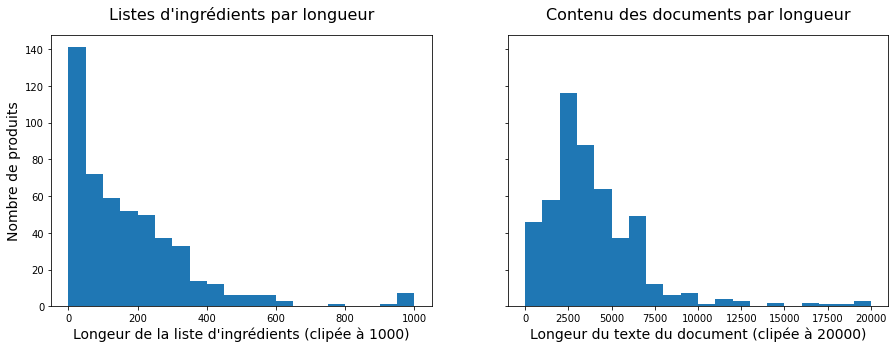
\includegraphics[width=0.9\linewidth]{img/text_lengths.png}
            \end{center}
            \caption{Distribution des longueurs de textes}
            \label{fig:text_length}
        \end{figure}     
        \begin{figure}[htbp]
            \begin{center}
            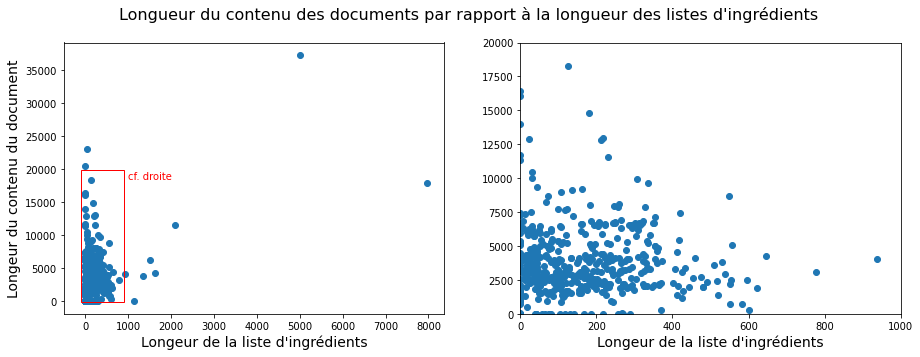
\includegraphics[width=0.9\linewidth]{img/text_lengths_2.png}
            \end{center}
            \caption{Corrélation entre longueurs des textes}
            \label{fig:text_length_2}
        \end{figure}     
        
        
    \chapter{Analyse textuelle}

        \section{Mots de chacun des corpus}

        Pour l'analyse des mots de chacun des corpus (listes d'ingrédients et contenu des documents), on fait d'abord un preprocessing de ces textes bruts :
        \begin{itemize}
            \item mise en minuscule de ces textes
            \item retrait des accents
            \item retrait des stopwords suivants : {'pas', 'le', 'en', 'pour', 'ou', 'ce', 'de', 'dans', 'du', 'and', 'un', 'sur', 'et', 'of', 'est', 'par', 'la', 'les', 'dont', 'au', 'des'}
            \item split des textes à chaque whitespace (espace, tabulation, retour à la ligne, \dots)
        \end{itemize}
        La liste de ces stopwords a été manuellement établie à partir des mots les plus fréquents de chacun des vocabulaires.
        Elle est commune aux deux corpus.
        Un descriptif des vocabulaires est présenté à la \reftable{tbl:vocabularies}.
        Un rapide parcours de ces exemples montre que l'utilisation des mots dans ces deux corpus (ingrédients et contenu des documents) est différente.
        On s'attend à pouvoir différencier automatiquement ces types de textes.
        Le vocabulaire des ingrédients est, comme on pouvait s'y attendre, entièrement inclus dans le vocabulaire du contenu des fiches techniques.
        
        {\renewcommand{\arraystretch}{1.5}%
        \begin{table}[htbp]
            \begin{center}
            {\scriptsize
            \begin{tabular}{lcc}
    \toprule
    {} &  \textbf{Ingrédients} &  \textbf{Contenu des documents} \\
    \midrule
    \textbf{Longueur du vocabulaire      } &  1324 & 15465 \\
    \hline
    \multirow{20}*{\textbf{Top 20 mots}} &sucre       : 363 occurences & produit     : 2198 occurences \\
    &acide       : 255 occurences & non         : 2164 occurences \\
    &sel         : 240 occurences & produits    : 1508 occurences \\
    &sirop       : 180 occurences & 10          : 1404 occurences \\
    &eau         : 178 occurences & kg          : 1290 occurences \\
    &poudre      : 176 occurences & base        : 1119 occurences \\
    &arome       : 175 occurences & sel         : 1041 occurences \\
    &lait        : 171 occurences & poids       : 1021 occurences \\
    &ble         : 171 occurences & 100         : 971 occurences \\
    &huile       : 146 occurences & palette     : 933 occurences \\
    &citrique    : 132 occurences & ingredients : 917 occurences \\
    &farine      : 128 occurences & date        : 904 occurences \\
    &amidon      : 125 occurences & sucre       : 841 occurences \\
    &glucose     : 124 occurences & 12          : 803 occurences \\
    &cacao       : 122 occurences & code        : 801 occurences \\
    &extrait     : 117 occurences & lait        : 733 occurences \\
    &acidifiant  : 114 occurences & absence     : 697 occurences \\
    &aromes      : 98 occurences & fiche       : 688 occurences \\
    &soja        : 96 occurences & the         : 658 occurences \\
    &concentre   : 92 occurences & france      : 657 occurences \\
    \bottomrule
\end{tabular}
            }
            \caption{Caractéristiques des vocabulaires}
            \label{tbl:vocabularies}
            \end{center}
        \end{table}
        }

        \section{Répartitions des mots dans et hors des listes d'ingrédients}

        On calcule la \og document frequency \fg des mots du corpus des ingrédients dans les listes d'ingrédients.
        Elle s'étend simplement au corpus du contenu des documents en la mettant à 0 pour les mots qui n'appartiennent pas au vocabulaire des ingrédients.
        Cela permet de calculer un score $s_{i}$ pour chaque mot $i$ via la formule suivante :
        \[s_{i} = \log_{2}(1 + c_{i})\]
        où $c_{i}$ est le nombre de listes d'ingrédients dans lequel le mot $i$ apparaît.
       
        Le score vaut donc $0$ si le mot n'est pas présent dans le vocabulaire des ingrédients, $1$ s'il est présent une fois, et progresse de manière logarithmique en fonction de la \og document frequency \fg. Une illustration est donnée à la \reffig{fig:scores_bar}

        \begin{figure}[htbp]
            \begin{center}
            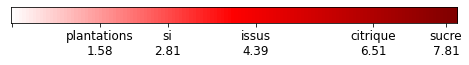
\includegraphics[width=0.6\linewidth]{img/scores_bar.png}
            \end{center}
            \caption{Exemple de scores de mots}
            \label{fig:scores_bar}
        \end{figure}

        \section{Représentations graphiques des textes et mots}

            \subsection{Vectorisation des mots}

            \subsection{Vectorisation des textes}